\documentclass{article}
\usepackage[T1]{fontenc}
\usepackage{lmodern}
\usepackage{graphicx}
\usepackage{amsmath,amssymb}
\usepackage[a4paper,margin=2cm]{geometry}
\usepackage[absolute,overlay]{textpos}
\setlength{\TPHorizModule}{1mm}
\setlength{\TPVertModule}{1mm}
\usepackage[indonesian]{babel}
\usepackage{hyperref}
\setlength{\emergencystretch}{2em}
\title{13-Algoritma-RSA-2026}
\author{pdf\_ppt\_to\_latex}
\date{}

\begin{document}

% --- unit llm 1 ---
% === Halaman 1 (llm) ===

\begin{center}
Bahan kuliah IF4020 Kriptografi

{\huge \color{red} 13 - Algoritma RSA}

\vspace{20mm}

Oleh: Rinaldi M

\vspace{10mm}

Program Studi Teknik Informatika\\
Sekolah Teknik Elektro dan Informatika\\
Institut Teknologi Bandung\\
2026
\end{center}

\newpage

% --- unit llm 2 ---
% === Halaman 2 (llm) ===

\section*{Pendahuluan}

\begin{itemize}
    \item RSA merupakan algoritma kunci-publik yang paling terkenal dan paling banyak aplikasinya.
    \item Dibuat oleh tiga peneliti dari \textit{MIT (Massachussets Institute of Technology)}, yaitu Ronald \textcolor{red}{Rivest}, Adi \textcolor{red}{Shamir}, dan Leonard \textcolor{red}{Adleman}, pada tahun 1976.
    \item RSA = Rivest-Shamir-Adleman
    \item Keamanan algoritma RSA terletak pada sulitnya memfaktorkan bilangan bulat yang besar menjadi faktor-faktor prima.
\end{itemize}

\newpage

% --- unit llm 3 ---
% === Halaman 3 (llm) ===

\vspace{132.46mm}

The authors of RSA: Rivest, Shamir and Adleman

\vspace{10mm}

dahulu

\vspace{10mm}

sekarang

% deskripsi: Foto hitam putih ketiga penulis RSA (Rivest, Shamir, Adleman) di masa muda mereka di depan papan tulis.
% bbox normalisasi: [0.0840, 0.0300, 0.4300, 0.4760]
\begin{textblock*}{72.66mm}(17.64mm,8.91mm)
\noindent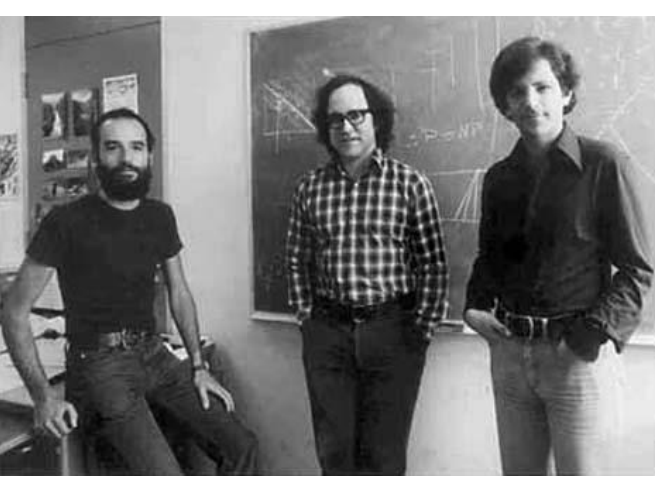
\includegraphics[width=72.66mm,height=132.46mm]{images/llm/page_003_img_01.png}%
\end{textblock*}

% deskripsi: Foto berwarna ketiga penulis RSA (Rivest, Shamir, Adleman) di masa tua mereka.
% bbox normalisasi: [0.5240, 0.3820, 0.9070, 0.8410]
\begin{textblock*}{80.43mm}(110.04mm,113.45mm)
\noindent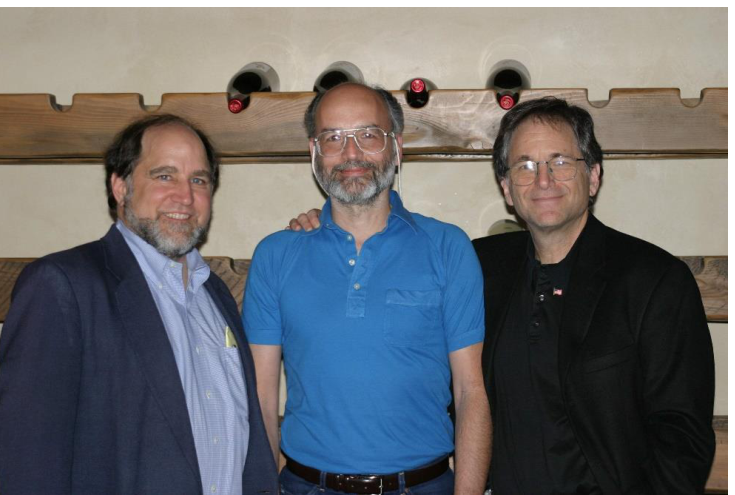
\includegraphics[width=80.43mm,height=136.32mm]{images/llm/page_003_img_02.png}%
\end{textblock*}

\newpage

% --- unit llm 4 ---
% === Halaman 4 (llm) ===

\section*{Properti Algoritma RSA}

\begin{enumerate}
    \item $p$ dan $q$ bilangan prima \hfill \textcolor{red}{(rahasia)}
    \item $n = p \cdot q$ \hfill (tidak rahasia)
    \item $\phi(n) = (p - 1)(q - 1)$ \hfill \textcolor{red}{(rahasia)}
    \item $e$ (kunci enkripsi) \hfill (tidak rahasia, disebut kunci publik)

    Syarat: $\text{PBB}(e, \phi(n)) = 1$, PBB = pembagi bersama terbesar = $gcd$

    \item $d$ (kunci dekripsi) \hfill \textcolor{red}{(rahasia, disebut kunci privat)}

    $d$ dihitung dari $d \equiv e^{-1} \pmod{\phi(n)}$

    \item $m$ (plainteks) \hfill \textcolor{red}{(rahasia)}
    \item $c$ (cipherteks) \hfill (tidak rahasia)
\end{enumerate}

\newpage

% --- unit llm 5 ---
% === Halaman 5 (llm) ===

\section*{Penurunan Rumus Enkripsi dan Dekripsi RSA}

\begin{itemize}
    \item Teori yang digunakan: Teorema Euler \[ a^{\phi(n)} \equiv 1 \pmod{n} \]
    \item Syarat:
    \begin{enumerate}
        \item $a$ harus relatif prima terhadap $n$, yaitu $\text{PBB}(a, n) = 1$ $\quad(\text{PBB} = gcd)$
        \item $\phi(n) = \text{Totient Euler} = \text{fungsi yang menentukan berapa banyak dari bilangan-bilangan } 1, 2, 3, \dots, n \text{ yang relatif prima terhadap } n.$
    \end{enumerate}
    
    Contoh: $\phi(20) = 8$, sebab terdapat 8 buah yang relatif prima dengan 20, yaitu $1, 3, 7, 9, 11, 13, 17, 19$.
\end{itemize}

Jika $n = pq$ adalah bilangan komposit dengan $p$ dan $q$ prima, maka
\[ \phi(n) = \phi(p) \phi(q) = (p - 1)(q - 1). \]

\newpage

% --- unit llm 6 ---
% === Halaman 6 (llm) ===

\begin{align*}
a^{\phi(n)} &\equiv 1 \pmod{n} \\
&\downarrow \text{ (pangkatkan kedua ruas dengan k)} \\
a^{k\phi(n)} &\equiv 1^k \pmod{n} \\
&\downarrow \\
a^{k\phi(n)} &\equiv 1 \pmod{n} \\
&\downarrow \text{ (ganti $a$ dengan $m$)} \\
m^{k\phi(n)} &\equiv 1 \pmod{n} \\
&\downarrow \text{ (kalikan kedua ruas dengan $m$)} \\
m^{k\phi(n)+1} &\equiv m \pmod{n}
\end{align*}

\newpage

% --- unit llm 7 ---
% === Halaman 7 (llm) ===

\begin{itemize}
  \item Misalkan $e$ dan $d$ dipilih sedemikian sehingga
  \[ e \cdot d \equiv 1 \pmod{\phi(n)} \]
  atau
  \[ e \cdot d = k\phi(n) + 1 \]
  Maka
  \[ m^{k\phi(n)+1} \equiv m \pmod{n} \]
  \vspace{5mm}
  \[ m^{e \cdot d} \equiv m \pmod{n} \longrightarrow (m^e)^d \equiv m \pmod{n} \]
  \vspace{5mm}
  \item Enkripsi: $c = E_e(m) = m^e \pmod{n}$
  \item Dekripsi: $m = D_d(c) = c^d \pmod{n}$
\end{itemize}

\vspace{32.97mm}

% deskripsi: Persamaan enkripsi RSA yang dilingkari kotak merah
% bbox normalisasi: [0.2470, 0.6340, 0.5300, 0.7450]
\begin{textblock*}{59.43mm}(51.87mm,188.30mm)
\noindent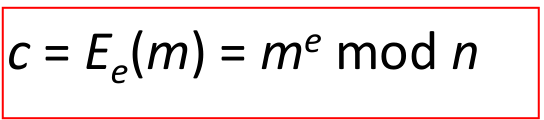
\includegraphics[width=59.43mm,height=32.97mm]{images/llm/page_007_img_01.png}%
\end{textblock*}

% deskripsi: Persamaan dekripsi RSA yang dilingkari kotak merah
% bbox normalisasi: [0.2470, 0.7610, 0.5320, 0.8720]
\begin{textblock*}{59.85mm}(51.87mm,226.02mm)
\noindent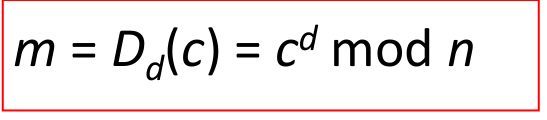
\includegraphics[width=59.85mm,height=32.97mm]{images/llm/page_007_img_02.png}%
\end{textblock*}

\newpage

% --- unit llm 8 ---
% === Halaman 8 (llm) ===

\section*{Prosedur Pembangkitan Sepasang Kunci}

\begin{enumerate}
  \item Pilih dua bilangan prima, $p$ dan $q$ (sebaiknya $p \neq q$)
  \item Hitung $n = pq$.
  \item Hitung $\phi(n) = (p-1)(q-1)$.
  \item Pilih sebuah bilangan bulat $e$ sebagai kunci publik, $e$ harus relatif prima terhadap $\phi(n)$.
  \item Hitung kunci dekripsi, $d$, dengan kekongruenan
  \[ ed \equiv 1 \pmod{\phi(n)} \text{ atau } d \equiv e^{-1} \pmod{\phi(n)} \to d = \frac{1+k\phi(n)}{e} \]
\end{enumerate}

Hasil dari algoritma di atas:
\begin{itemize}
  \item Kunci publik adalah pasangan $(e, n)$
  \item Kunci privat adalah pasangan $(d, n)$
\end{itemize}

\newpage

% --- unit llm 9 ---
% === Halaman 9 (llm) ===

\section*{Enkripsi}

\begin{enumerate}
    \item \textit{Preprocessing}: Pesan yang akan dienkripsi dikodekan menjadi integer $m$. Jika $m$ berukuran besar, pecah $m$ menjadi blok-blok plainteks yang lebih kecil: $m_1, m_2, m_3, \dots$ (syarat: $0 \le m_i < n - 1$)
    \item Hitung cipherteks $c$ untuk plainteks $m$ menggunakan kunci publik $e$ dengan persamaan
    \[ c = m^e \text{ mod } n \]
    Jika $m$ dipecah menjadi $m_1, m_2, m_3, \dots$, enkripsi setiap $m_i$ menjadi
    \[ c_i = m_i^e \text{ mod } n \]
\end{enumerate}

\newpage

% --- unit llm 10 ---
% === Halaman 10 (llm) ===

\section*{Dekripsi}

\begin{enumerate}
    \item Hitung kembali blok plainteks $m$ dari cipherteks $c$ menggunakan kunci privat $d$ dengan persamaan
    \[ m = c^d \pmod{n}, \]
    Jika cipherteks adalah blok $c_1, c_2, c_3, \dots$, dekripsi setiap blok menjadi
    \[ m_i = c_i^d \pmod{n} \]
    
    \item \textbf{Postprocessing}: Kodekan kembali $m$ atau $m_i$ menjadi bentuk pesan semula
\end{enumerate}

\newpage

% --- unit llm 11 ---
% === Halaman 11 (llm) ===

\section*{Contoh pembangkitan kunci oleh Alice}

\begin{itemize}
    \item Misalkan Alice ingin menghitung pasangan kunci publik dan kunci privatnya.
    \item Misalkan Alice memilih $p = 47$ dan $q = 71$ (keduanya prima), maka dapat dihitung:
    \[ n = p \times q = 3337 \]
    \[ \phi(n) = (p - 1) \times (q - 1) = (47 - 1)(71 - 1) = 46 \times 60 = 3220. \]
    \item Alice memilih kunci publik $e = 79$ (yang relatif prima dengan 3220 karena pembagi bersama terbesarnya adalah 1).
    \item Kunci publik Alice adalah $(e, n) = (79, 3337)$. Nilai $e$ dan $n$ dapat dipublikasikan kepada umum.
\end{itemize}

\newpage

% --- unit llm 12 ---
% === Halaman 12 (llm) ===

\begin{itemize}
    \item Selanjutnya Alice menghitung kunci privat $d$ dengan kekongruenan:
    \[ ed \equiv 1 \pmod{\phi(n)} \longrightarrow d = \frac{1 + k \phi(n)}{e} \]
    $d$ adalah balikan $e$ dalam modulus $\phi(n)$ \\
    $d$ dapat dihitung dengan dengan rumus:
    \[ d = \frac{1 + k\phi(n)}{e} = \frac{1 + 3220k}{79} \]
    \vspace{5mm}
    Coba berbagai nilai-nilai $k = 1, 2, 3, \dots$, sampai mendapatkan $d$ bilangan bulat:
    \begin{align*}
        k = 1 & \rightarrow d = (1 + 3220 \times 1)/79 = 3221/79 = 40,77 & \text{(bukan bilangan bulat)}
        k = 2 & \rightarrow d = (1 + 3220 \times 2)/79 = 6441/79 = 81,53 & \text{(bukan bilangan bulat)}
        k = \dots & \text{dst}
    \end{align*}
    \textbf{k = 25 $\rightarrow$ d = (1 + 3220 $\times$ 25)/79 = 80501/79 = 1019 (bilangan bulat)}
    \newline diperoleh nilai $d$ yang bulat adalah 1019. Ini adalah kunci privat.
    \item Jadi, kunci privat Alice adalah $(d, n) = (1019, 3337)$. \textcolor{red}{Keep them secret!}
\end{itemize}

\newpage

% --- unit llm 13 ---
% === Halaman 13 (llm) ===

\section*{Contoh pengiriman pesan 1:}

\begin{itemize}
    \item Misalkan Bob mengirim pesan $m = 16$ kepada Alice. Bob mengenkripsi $m$ dengan kunci publik Alice $(e, n) = (79, 3337)$ sebagai berikut:
    \[ c = m^e \text{ mod } n = 16^{79} \text{ mod } 3337 = 1493 \]
    
    Bob mengirim $c = 1493$ kepada Alice
    
    \item Alice mendekripsi cipherteks $c = 1493$ dengan kunci privat miliknya, yaitu $(d, n) = (1019, 3337)$ sebagai berikut:
    \[ m = c^d \text{ mod } n = 1493^{1019} \text{ mod } 3337 = 16 \]
    
    Alice mendapatkan kembali plainteks dari Bob, yaitu $m = 16$
\end{itemize}

\newpage

% --- unit llm 14 ---
% === Halaman 14 (llm) ===

\section*{Contoh pengiriman pesan 2:}
\begin{itemize}
    \item Misalkan Bob akan mengirim plainteks $M = \text{'HELLO ALICE'}$ kepada Alice
    \item Dengan memisalkan $\text{A} = 00, \text{B} = 01, \dots, \text{Z} = 25$, maka plainteks dikodekan ke dalam \textit{integer} (spasi diabaikan) menjadi
    \[ m = 070411111140011080204 \]
\end{itemize}

Nilai $m$ ini sangat besar untuk dipangkatkan dan tidak berada di dalam selang $[0, 3337-1]$, oleh karena itu pecah $m$ menjadi blok-blok pesan yang lebih kecil, misalnya blok 4 digit:

\begin{align*}
    m_1 &= 0704 & m_4 &= 1108 \\
    m_2 &= 1111 & m_5 &= 0204 \\
    m_3 &= 1400 & \\
\end{align*}

(Perhatikan, $m_i$ masih valid karena terletak di dalam selang $[0, 3337 - 1])$

\newpage

% --- unit llm 15 ---
% === Halaman 15 (llm) ===

\begin{flushright}
\fbox{Enkripsi: $c = m^e \pmod{n}$}
\end{flushright}

\begin{itemize}
    \item Bob mengenkripsi setiap blok plainteks dengan menggunakan kunci publik Alice ($e = 79$, $n = 3337$):
    \begin{align*}
        m_1 = 0704 & \to c_1 = 704^{79} \pmod{3337} = 328; \\
        m_2 = 1111 & \to c_2 = 1111^{79} \pmod{3337} = 301; \\
        m_3 = 1400 & \to c_3 = 1400^{79} \pmod{3337} = 2653; \\
        m_4 = 1108 & \to c_4 = 1108^{79} \pmod{3337} = 2986; \\
        m_1 = 204 & \to c_5 = 204^{79} \pmod{3337} = 1164;
    \end{align*}

    Cipherteks: $C = 0328, 0301, 2653, 2986, 1164$

    \item Bob mengirim cipherteks $C$ kepada Alice
\end{itemize}

\newpage

% --- unit llm 16 ---
% === Halaman 16 (llm) ===

\begin{flushright}\fbox{Dekripsi: $m = c^d \pmod{n}$}\end{flushright}

\begin{itemize}
    \item Alice mendekripsi cipherteks $C = 0328, 0301, 2653, 2986, 1164$ dengan menggunakan kunci privatnya, yaitu $d = 1019, n = 3337$:
    
    \begin{align*}
    c_1 = 0328 \rightarrow m_1 &= 328^{1019} \pmod{3337} = 704 = 0704 \\
    c_2 = 0301 \rightarrow m_2 &= 301^{1019} \pmod{3337} = 1111 \\
    c_3 = 2653 \rightarrow m_3 &= 2653^{1019} \pmod{3337} = 1400 \\
    c_4 = 2986 \rightarrow m_4 &= 2986^{1019} \pmod{3337} = 1108 \\
    c_5 = 1164 \rightarrow m_5 &= 1164^{1019} \pmod{3337} = 204
    \end{align*}
    
    \item Alice memperoleh kembali plainteks dari Bob \\ $m = 07041111140011080204$
\end{itemize}

yang dikodekan kembali (A = 00, B = 01, C = 02, ..., Z = 25) menjadi \\ $M = \text{HELLO ALICE}$

\newpage

% --- unit llm 17 ---
% === Halaman 17 (llm) ===

\section*{Keamanan RSA}

\begin{itemize}
    \item Keamanan algoritma $RSA$ terletak pada tingkat kesulitan dalam memfaktorkan bilangan bulat $n$ faktor-faktor prima ($p$ dan $q$), yang dalam hal ini $n = p \times q$. Semakin besar $n$, semakin sulit difaktorkan.
    \item Sekali $n$ berhasil difaktorkan menjadi $p$ dan $q$, maka
    \[ \phi(n) = (p - 1) \times (q - 1) \text{ dapat dihitung.} \]
    Selanjutnya, karena kunci enkripsi $e$ diumumkan (tidak rahasia), maka kunci dekripsi $d$ dapat dihitung dari kekongruenen
    \[ ed \equiv 1 \pmod{\phi(n)} \rightarrow d = \frac{1 + k \, \phi(n)}{e} \]
\end{itemize}

\newpage

% --- unit llm 18 ---
% === Halaman 18 (llm) ===

\begin{itemize}
    \item Penemu algoritma $RSA$ pada tahun 1976 menyarankan nilai $p$ dan $q$ panjangnya lebih dari 100 digit. Dengan demikian hasil kali $n = p \times q$ akan berukuran lebih dari 200 digit.
    \item Usaha untuk mencari faktor bilangan 200 digit membutuhkan waktu komputasi selama 4 milyar tahun, sedangkan untuk bilangan 500 digit membutuhkan waktu $10^{25}$ tahun (dengan asumsi bahwa algoritma pemfaktoran yang digunakan adalah algoritma yang tercepat saat ini dan komputer yang dipakai mempunyai kecepatan 1 milidetik).
    \item Algoritma pemfaktoran yang tercepat saat ini memiliki kompleksitas
    \[ O(\exp(\sqrt[3]{\frac{64}{9}}b(\log(b)^2))) \]
    untuk bilangan bulat $n$ sepanjang b-bit.
\end{itemize}

\newpage

% --- unit llm 19 ---
% === Halaman 19 (llm) ===

\begin{itemize}
  \item Hingga saat ini belum ditemukan algoritma pemfaktoran bilangan bulat besar dalam waktu polinomial.
  \item Fakta inilah yang membuat algoritma $RSA$ dianggap masih aman untuk saat ini. Semakin panjang bilangan bulatnya, maka semakin lama waktu yang dibutuhkan untuk memfaktorkannya.
  \item Namun jika komputer kuantum semakin maju dan berkembang, maka algoritma RSA akan terancam, sebab $n$ dapat difaktorkan dengan komputasi kuantum. Algoritma berbasis komputasi kuantum yang dapat memfaktorkan $n$ dalam waktu polinom adalah algoritma $Shor$.
\end{itemize}

\newpage

% --- unit llm 20 ---
% === Halaman 20 (llm) ===

\section*{Contoh parameter RSA}

\begin{itemize}
    \item Modulus $n$ sepanjang 1024 bit (setara 300 angka decimal)
    \item Bilangan prima $p$ dan $q$ masing-masing panjangnya sekitar 154 angka decimal
    \item Sumber: \url{https://www.di-mgt.com.au/rsa_alg.html}
\end{itemize}

\begin{itemize}
    \item $n = $\
    \begin{align*}
    &1192941348401695090555272113312556496446065696615276380120674819549430568 \\
    &511503380631595703771562029703500011862877084668996911289221224545711806 \\
    &057499598951708004210526342736322274266393116193517839570773505632231596 \\
    &6811219273374739732203125125990612313222509455062600665575382385175753906 \\
    &21262940383913963
    \end{align*}

    \item $p = $\
    \begin{align*}
    &1093376618363257581761151703473066828715579998463222345413874567112127345 \\
    &6287670008290843302875521274970245314593222946129064538358581018615539828 \\
    &479146469
    \end{align*}

    \item $q = $\
    \begin{align*}
    &1091061696734911023172373407861492264533706088214174896820983422513897601 \\
    &1179993394299810159736904468554021708289824396553412180514827996444845438 \\
    &176099727
    \end{align*}
\end{itemize}

\newpage

% --- unit llm 21 ---
% === Halaman 21 (llm) ===

\begin{itemize}
    \item Secara umum dapat disimpulkan bahwa RSA hanya aman jika $n$ cukup besar.
    \item Jika panjang $n$ hanya 256 bit atau kurang, ia dapat difaktorkan dalam beberapa jam saja dengan sebuah komputer $PC$ dan program yang tersedia secara bebas.
    \item Jika panjang $n$ adalah 512 bit atau kurang, ia dapat difaktorkan dengan beberapa ratus komputer.
    \item Saat ini panjang kunci RSA yang aman adalah jika $n$ di atas 1024 bit.
\end{itemize}

\newpage

% --- unit llm 22 ---
% === Halaman 22 (llm) ===

\begin{itemize}
    \item Tahun 1977, 3 orang penemu $RSA$ membuat sayembara untuk memecahkan cipherteks dengan menggunakan RSA di majalah \textit{Scientific American}.
    \item Hadiahnya: \$100
    \item Tahun 1994, kelompok yang bekerja dengan kolaborasi internet berhasil memecahkan cipherteks hanya dalam waktu 8 bulan.
\end{itemize}

\newpage

% --- unit llm 23 ---
% === Halaman 23 (llm) ===

\section*{Kelemahan RSA}

\begin{itemize}
    \item RSA lebih lambat daripada algoritma kriptografi kunci-simetri seperti $DES$ dan $AES$
    \item Dalam praktek, $RSA$ tidak digunakan untuk mengenkripsi pesan yang berukuran besar, tetapi digunakan untuk mengenkripsi kunci simetri (kunci sesi) dengan menggunakan kunci publik penerima pesan. Karena, kunci simeteri umumnya relative pendek.
    \item Pesan tetap dienkripsi dengan algoritma simetri seperti $DES$ atau $AES$.
    \item Pesan dan kunci simetri (yang terenkripsi) dapat dikirim bersamaan. Penerima mendekripsi kunci simetri dengan kunci privatnya, lalu mendekripsi pesan dengan kunci simetri tersebut.
    \item Kombinasi kedua system kriptografi ini (simeteri dan nirsimetri) dinamakan \textit{hybrid cryptography}.
\end{itemize}

\newpage

% --- unit llm 24 ---
% === Halaman 24 (llm) ===

\section*{Man-in-the-middle Attack}

\begin{itemize}
    \item Karena pengirim dan penerima harus berbagi kunci publik, maka distribusi kunci publik dapat mengalami serangan \textit{man-in-the-middle attack}.
    \item Misalkan Alice dan Bob mengirim kunci publiknya masing-masing melalui saluran komunikasi. Orang-di-tengah, misalkan Carol, mengintersepsi komunikasi antara Bob dan Alice lalu ia berpura-pura sebagai salah satu pihak (Alice atau Bob).
    \item Carol (yang menyamar sebagai Alice) mengirim kunci publiknya kepada Bob (Bob percaya itu adalah kunci publik Alice), dan Carol (yang menyamar sebagai Bob) mengirim kunci publiknya kepada Alice (Alice percaya itu adalah kunci publik Bob).
    \item Selanjutnya, Carol mendekripsi pesan dari Bob dengan kunci privatnya, menyimpan salinannya, lalu mengenkripsi pesan tersebut dengan kunci publik Alice, dan mengirim cipherteks tersebut kepada Alice. Alice dan Bob tidak dapat mendeteksi keberadaan Carol.
\end{itemize}

\newpage

% --- unit llm 25 ---
% === Halaman 25 (llm) ===

\section*{Public-Key Encryption by RSA Algorithm}

\subsection*{Objective}
The purpose of this page is to demonstrate step by step how a public-key encryption system works. We use the RSA algorithm (named after the inventors Rivest, Shamir, Adleman) with very small primes. The basic functions are implemented in JavaScript and can be viewed in the source.

\textbf{Note:} This page is only for explaining the mechanism. In practice more advanced algorithms and much larger primes are used!

\subsection*{Overview}
Working with a public-key encryption system has mainly three phases:

\begin{enumerate}
    \item \textbf{Key Generation:} Whoever wants to receive secret messages creates a public key (which is published) and a private key (kept secret). The keys are generated in a way that conceals their construction and makes it 'difficult' to find the private key by only knowing the public key.
    \item \textbf{Encryption:} A secret message to any person can be encrypted by his/her public key (that could be officially listed like phone numbers).
    \item \textbf{Decryption:} Only the person being addressed can easily decrypt the secret message using the private key.
\end{enumerate}

\subsection*{RSA Key Generation}
From two selected primes the computer will generate the public and the private key:

Pick 2 (different) primes: $p = 7$ $\quad q = 11$ \vspace{10mm}

\vspace{35.64mm}

\begin{align*}
    n &= 77 && (n = p.q) \\
    \varphi &= 60 && (\varphi = \varphi(n) = (p-1).(q-1); \text{ needed to determine e and d}) \\
    e &= 7 && (\text{arbitrary, but less than n and relatively prime to } \varphi)
\end{align*}

% deskripsi: Screenshot area input interaktif untuk pemilihan bilangan prima p dan q serta tombol Generate keys
% bbox normalisasi: [0.1500, 0.7800, 0.3900, 0.8400]
\begin{textblock*}{50.40mm}(31.50mm,231.66mm)
\noindent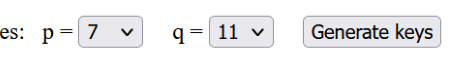
\includegraphics[width=50.40mm,height=17.82mm]{images/llm/page_025_img_01.png}%
\end{textblock*}

% deskripsi: Screenshot area output kalkulasi nilai n, phi, dan e dalam proses pembuatan kunci RSA
% bbox normalisasi: [0.3400, 0.8400, 0.7100, 0.9600]
\begin{textblock*}{77.70mm}(71.40mm,249.48mm)
\noindent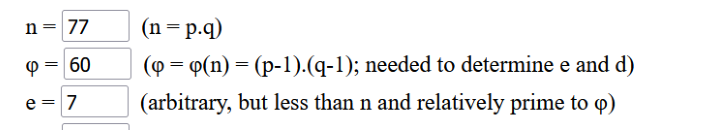
\includegraphics[width=77.70mm,height=35.64mm]{images/llm/page_025_img_02.png}%
\end{textblock*}

\newpage

% --- unit llm 26 ---
% === Halaman 26 (llm) ===

\section*{RSA Encryption}

First of all we need the public key of the person to whom we want to send the message:

$(e, n) = (7, 77)$ (Enter appropriate values or Take public key from above)

Next we need the message. For simplicity let us demonstrate this here with just one letter. (In secure applications letters are never encrypted individually, but in whole blocks.)

Pick a letter to cipher: H

Before we can encrypt this letter we must encode it as a number:

$m = 8$ (here we take just the index in the alphabet)

Encryption itself is very simple: $m' = 57$ \[ (m' = m^e \pmod n) \]

The value $m'$ is the encrypted message sent to the receiver.

\vspace{10mm}

\section*{RSA Decryption}

First of all we need the private key of the person who got the encrypted message:

$(d, n) = (43, 77)$ (Enter appropriate values or Take private key from above)

Next we need the encrypted message:

$m' = 57$ (Enter an appropriate value or Take encrypted message from above)

Decryption again is very simple: $m = 8$ \[ (m = m'^d \pmod n) \]

The decoded message should match with the above chosen letter: H

\newpage

% --- unit llm 27 ---
% === Halaman 27 (llm) ===

\section*{Public Key Cryptography using RSA algorithm}
by: Syed Umar Anis

Purpose of the page is to demonstrate how RSA algorithm works - generates keys, encrypts message and decrypts it.

See the related blog post for more explanation.

\vspace{10mm}

\subsection*{Step \# 1: Generate Private and Public keys}

Enter two prime numbers below (P, Q), then press calculate:

\begin{itemize}
    \item P: 17
    \item Q: 29
\end{itemize}

\vspace{56.43mm}

Some prime numbers: 11, 13, 17, 19, 23, 29, 191, 193, 197, 199, etc.

\vspace{5mm}

% deskripsi: Tabel kalkulasi RSA yang menunjukkan variabel N (modulus) dan L (length) beserta nilai, nama, formula, dan deskripsinya.
% bbox normalisasi: [0.0400, 0.7800, 0.9500, 0.9700]
\begin{textblock*}{191.10mm}(8.40mm,231.66mm)
\noindent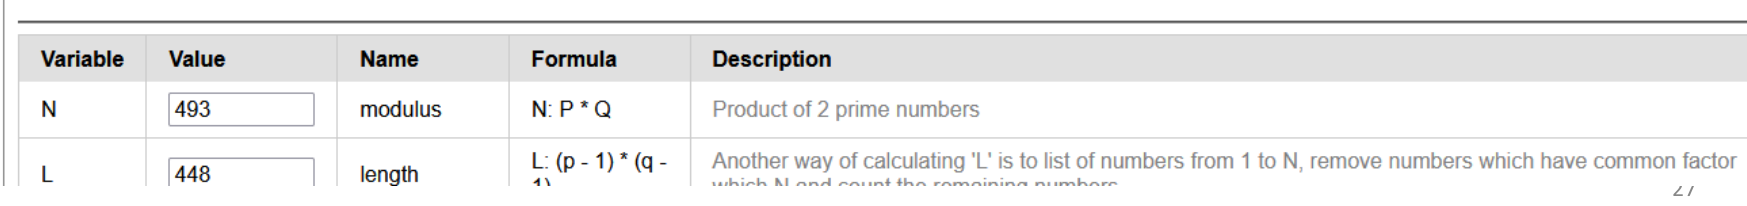
\includegraphics[width=191.10mm,height=56.43mm]{images/llm/page_027_img_01.png}%
\end{textblock*}

\newpage

% --- unit llm 28 ---
% === Halaman 28 (llm) ===

\vspace{243.54mm}

Demo Online RSA 3: \url{https://www.lddgo.net/en/encrypt/rsa}

% deskripsi: Screenshot antarmuka situs web RSA Encryption and Decryption Online yang menunjukkan kolom Input Content, Input Key, dan berbagai opsi pengaturan enkripsi seperti Mode (ECB), Padding (PKCS1Padding), dan Key Type (Private Key).
% bbox normalisasi: [0.0400, 0.1400, 0.9500, 0.9600]
\begin{textblock*}{191.10mm}(8.40mm,41.58mm)
\noindent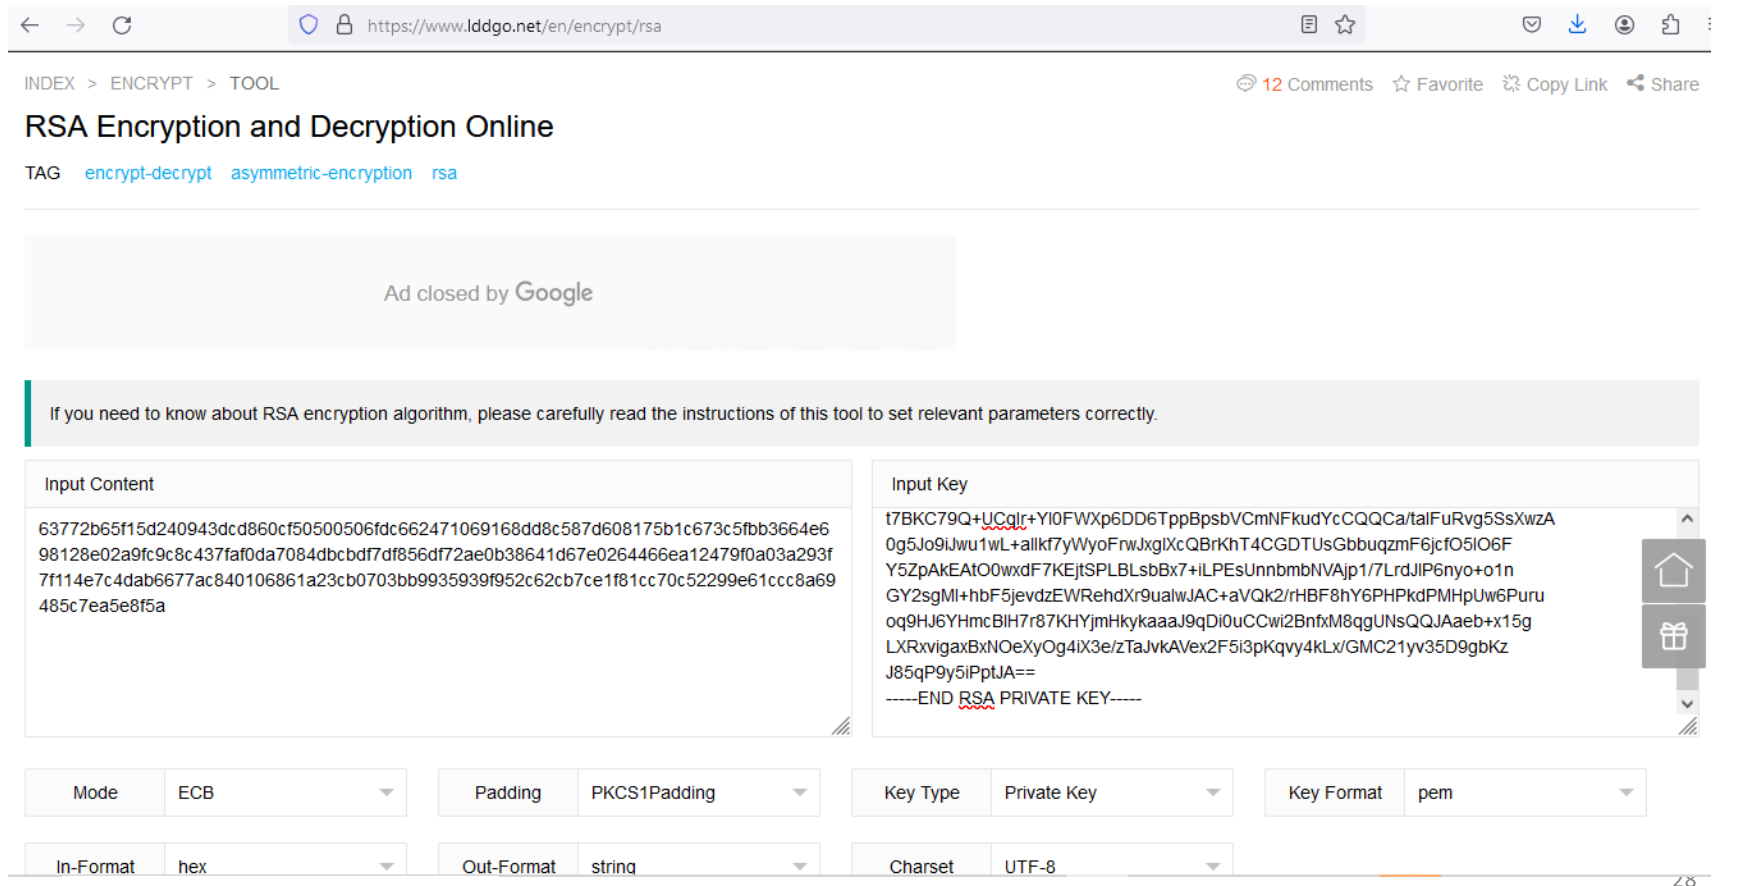
\includegraphics[width=191.10mm,height=243.54mm]{images/llm/page_028_img_01.png}%
\end{textblock*}

\newpage

% --- unit llm 29 ---
% === Halaman 29 (llm) ===

\section*{Kode Program RSA dalam Bahasa Python}

\begin{enumerate}
    \item Kode program enkripsi dan dekripsi pesan dengan kunci publik dan kunci privat milik sendiri, di dalamnya termasuk:
    \begin{itemize}
        \item mensimulasikan perhitungan kunci publik dan kunci privat
    \end{itemize}
    \item Kode program enkripsi dan dekripsi pesan dengan kunci publik dan kunci privat milik sendiri, di dalamnya termasuk:
    \begin{itemize}
        \item membangkitkan kunci publik dan kunci privat dengan fungsi RSA.generate()
        \item Kunci publiK dan kunci privat disimpan di dalam file dengan format PEM
    \end{itemize}
    \item Kode program enkripsi pesan dengan kunci publik pengirim (Bob) dan dekripsi pesan dengan kunci privat penerima pesan (Alice)
\end{enumerate}

\newpage

% --- unit llm 30 ---
% === Halaman 30 (llm) ===

\section*{1. Kode Program RSA (1)}

\begin{verbatim}
from Crypto.PublicKey import RSA
from Crypto.Cipher import PKCS1_OAEP
from Crypto.Util.number import getPrime, inverse

def PembangkitanKunciRSA():
    key_size = 1024    # Gunakan 1024-bit untuk menghindari error
    p = getPrime(key_size // 2)
    q = getPrime(key_size // 2)
    n = p * q
    phi_n = (p - 1) * (q - 1)

    e = 65537    # Kunci publik, default, bisa diganti
    d = inverse(e, phi_n)    # Kunci privat

    # Buat kunci RSA
    key = RSA.construct((n, e, d, p, q))
\end{verbatim}

\newpage

% --- unit llm 31 ---
% === Halaman 31 (llm) ===

\begin{verbatim}
# Bungkus kunci dalam format PKCS1_OAEP untuk padding
public_key = PKCS1_OAEP.new(key.publickey())
private_key = PKCS1_OAEP.new(key)

# Tampilkan informasi kunci
print("Modulus (n):", key.n)
print("Kunci publik (e):", key.e)
print("Kunci privat (d):", key.d)
print("Bilangan prima p:", key.p)
print("Bilangan prima q:", key.q)

return public_key, private_key

def encrypt_message(message, public_key):
    #Enkripsi pesan dengan PKCS1_OAEP
    return public_key.encrypt(message.encode())

def decrypt_message(ciphertext, private_key):
    #Dekripsi pesan dengan PKCS1_OAEP
    return private_key.decrypt(ciphertext).decode()
\end{verbatim}

\newpage

% --- unit llm 32 ---
% === Halaman 32 (llm) ===

\begin{verbatim}
# Program utama

\vspace{127.71mm}

public_key, private_key = PembangkitanKunciRSA()

pesan = input("Ketikkan pesan teks: ")

ciphertext = encrypt_message(pesan, public_key)
print("\nCiphertext:", ciphertext.hex())

decrypted_message = decrypt_message(ciphertext, private_key)
print("\nPesan setelah dekripsi:", decrypted_message)
\end{verbatim}

% deskripsi: Screenshot potongan kode program Python untuk implementasi enkripsi dan dekripsi RSA.
% bbox normalisasi: [0.1100, 0.1400, 0.7800, 0.5700]
\begin{textblock*}{140.70mm}(23.10mm,41.58mm)
\noindent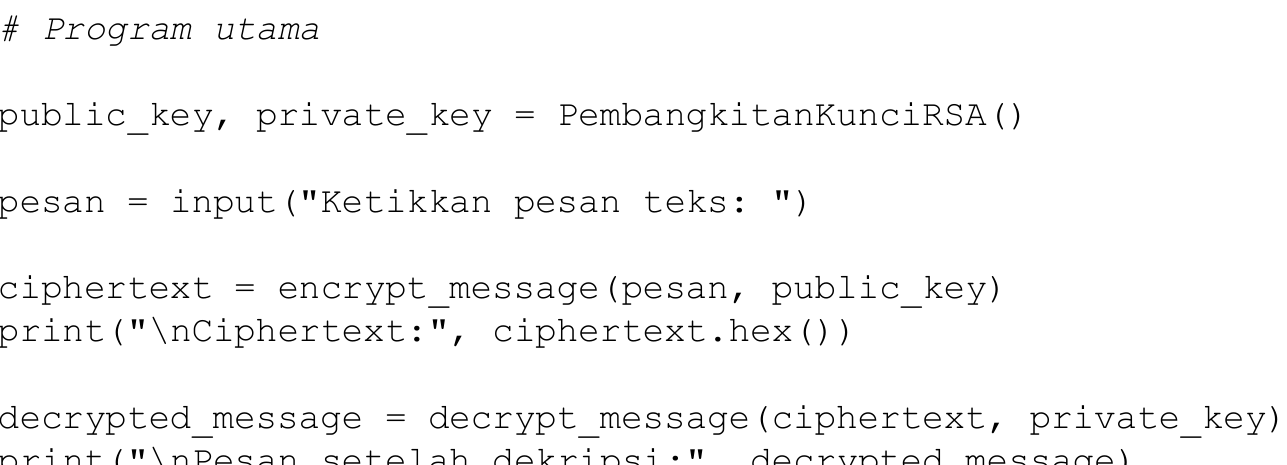
\includegraphics[width=140.70mm,height=127.71mm]{images/llm/page_032_img_01.png}%
\end{textblock*}

\newpage

% --- unit llm 33 ---
% === Halaman 33 (llm) ===

\textbf{Keterangan:}
\begin{itemize}
    \item PKCS \#1-OAEP adalah singkatan dari \textit{Public-Key Cryptography Standards \#1 -- Optimal Asymmetric Encryption Padding}.
    \item Jadi PKCS1\_OAEP merujuk pada skema \textit{padding} yang digunakan pada enkripsi RSA agar lebih aman.
\end{itemize}

\begin{enumerate}
    \item PKCS \#1
    \begin{itemize}
        \item PKCS \#1 adalah standar kriptografi yang mendefinisikan bagaimana algoritma RSA digunakan.
        Standar ini dibuat oleh RSA Laboratories dan berisi spesifikasi untuk:
        \begin{itemize}
            \item Enkripsi RSA
            \item Tanda tangan digital RSA
            \item Format kunci
            \item Skema \textit{padding}
        \end{itemize}
    \end{itemize}
\end{enumerate}

\newpage

% --- unit llm 34 ---
% === Halaman 34 (llm) ===

2. OAEP (\textit{Optimal Asymmetric Encryption Padding})
\begin{itemize}
    \item OAEP adalah metode \textit{padding} yang ditambahkan ke pesan sebelum dienkripsi dengan RSA.
    \item \textit{Padding} diperlukan karena:
    \begin{itemize}
        \item RSA tidak boleh mengenkripsi pesan langsung
        \item Tanpa \textit{padding}, RSA rentan terhadap berbagai serangan kriptografi
    \end{itemize}
    \item OAEP membuat pesan menjadi acak (\textit{randomized}) sebelum dienkripsi RSA, sehingga aman terhadap \textit{chosen-ciphertext attack}
    \begin{itemize}
        \item Skema ini diperkenalkan oleh Mihir Bellare dan Phillip Rogaway pada tahun 1994.
    \end{itemize}
    \item Pesan M sebelum dienkripsi RSA diproses sebagai berikut:
    \[ M \rightarrow OAEP\ padding \rightarrow encoded\ message \rightarrow RSA\ encryption \]
    \item Sehingga \textit{ciphertext} menjadi tidak deterministik (setiap enkripsi berbeda walaupun pesannya sama).
\end{itemize}

\newpage

% --- unit llm 35 ---
% === Halaman 35 (llm) ===

\textcolor{red}{\huge Hasil run program:}

Modulus (n):

107105801666381874958816898107516567038215030833881286317442333643278857794209843929433502698599718426847\n47896064453002989011854010624540750250536568182920407035631068956453823473995678447677208125743590950090093\n164725147330391992415298813450323789112371175324864721150342209300455286955187071194005483849

Kunci publik (e): 65537

Kunci privat (d):

886596844591790172200793664225289130747870140878252891995686336115702394121390793037782869603643595941934552\n3496063225337527459891829054790627538808857412268882775492783563147682092928066546646858718829012169421606174\n9593354172220122477067654187264109700360834353158767529592710050174332150940324547189793473

Bilangan prima p:

121153456200267798761827165740556977111024738980732444383114395825839460060498684419877671061047345501943836\n42530988866326301487387700105134589398882962009

Bilangan prima q:

8840506634972987516522193798981655080212041703435795849600206015029840825794928493482108794557350902986290324\n482043250339520205445179047843976171822356752761

Ketikkan pesan teks: Baru-baru ini gempa dengan magnitudo 7,8 terjadi di negara Myanmar

Ciphertext:

79b5dc24a495089df2b05c336381c6cde964f6fd040cf1e97b83c3d9989998a29ebe0d2370248ab89458141a71a7a0f4c571cb4048aefe2d6\n9500c0509e1732567bd5bde4109cb75e73cefc20b79863fa9af2b8d07930e36d33e5f602070291e0eaa2831448bed53bdfefd5be19bbb\nb39afdd86ebca04s54a2065a5b575389c

Pesan setelah dekripsi: Baru-baru ini gempa dengan magnitudo 7,8 terjadi di negara Myanmar

\newpage

% --- unit llm 36 ---
% === Halaman 36 (llm) ===

\section*{2. Kode Program RSA Python (2)}

\begin{verbatim}
from Crypto.PublicKey import RSA
from Crypto.Cipher import PKCS1_OAEP

def PembangkitanKunciRSA():
    # Buat kunci RSA
    key = RSA.generate(1024)
    kunci_publik = key.pubkey()

    # Tampilkan informasi kunci
    print("Modulus (n):", key.n)
    print("Kunci publik (e):", key.e)
    print("Kunci privat (d):", key.d)
    print("Bilangan prima p:", key.p)
    print("Bilangan prima q:", key.q)

    # Simpan kunci publik dan kunci privat ke dalam dua file kunci berbeda dengan format PEM
    with open("kunci_publik.pem", "wb") as file:
        file.write(kunci_publik.exportKey('PEM'))
        file.close()

    with open("kunci_privat.pem", "wb") as file:
        file.write(key.exportKey('PEM','passwordku'))  # Password bisa diubah
        file.close()
\end{verbatim}

\newpage

% --- unit llm 37 ---
% === Halaman 37 (llm) ===

\vspace{201.96mm}

\begin{verbatim}
def encrypt_message(message, file_kunci):
    #Enkripsi pesan
    with open(file_kunci, "rb") as file:
        kunci_publik = RSA.importKey(file.read())

    RSA_cipher = PKCS1_OAEP.new(kunci_publik)
    ciphertext = RSA_cipher.encrypt(message.encode())
    return ciphertext

def decrypt_message(ciphertext, file_kunci):
    #Dekripsi pesan
    with open(file_kunci, "rb") as file:
        kunci_privat = RSA.importKey(file.read(), 'passwordku')

    RSA_cipher = PKCS1_OAEP.new(kunci_privat)
    plaintext = RSA_cipher.decrypt(ciphertext)
    return plaintext
\end{verbatim}

% deskripsi: Screenshot potongan kode pemrograman Python untuk proses enkripsi dan dekripsi pesan menggunakan algoritma RSA.
% bbox normalisasi: [0.0900, 0.1000, 0.6800, 0.7800]
\begin{textblock*}{123.90mm}(18.90mm,29.70mm)
\noindent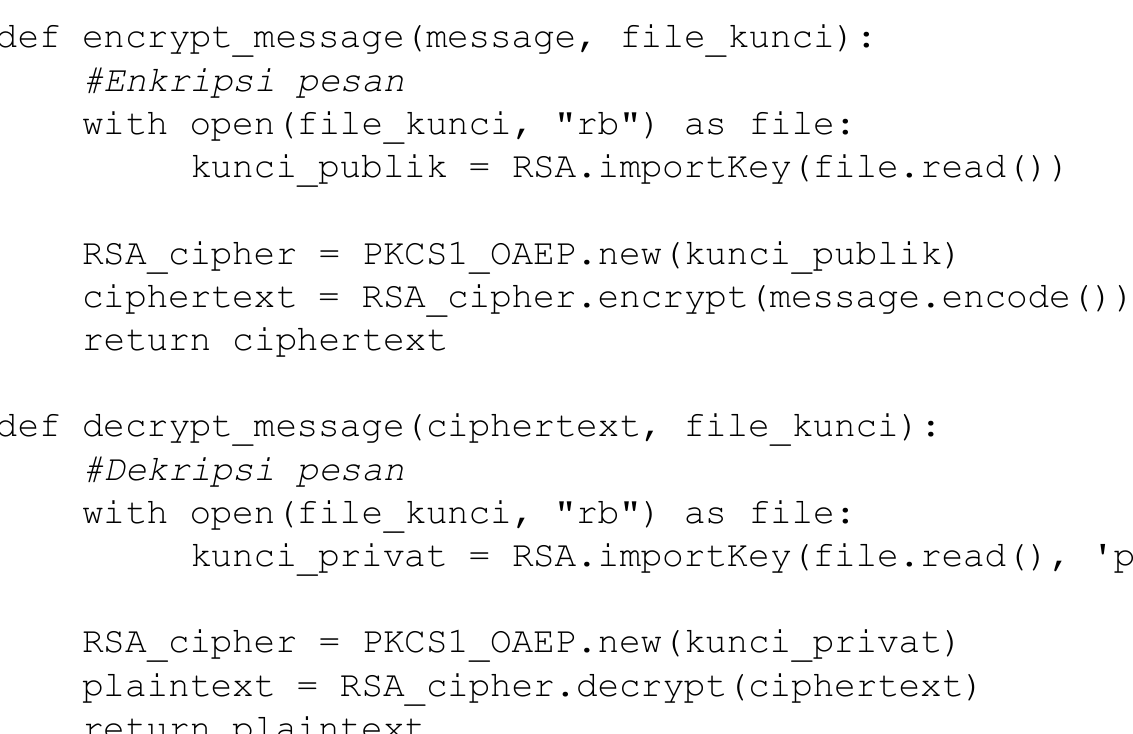
\includegraphics[width=123.90mm,height=201.96mm]{images/llm/page_037_img_01.png}%
\end{textblock*}

\newpage

% --- unit llm 38 ---
% === Halaman 38 (llm) ===

# Program utamaPembangkitanKunciRSA()

\vspace{86.13mm}

\begin{verbatim}
pesan = input("Ketikkan pesan teks: ")
ciphertext = encrypt_message(pesan, 'kunci_publik.pem')
print("\nCiphertext:", ciphertext.hex())

decrypted_message = decrypt_message(ciphertext, 'kunci_privat.pem')
print("\nPesan setelah dekripsi:", decrypted_message)
\end{verbatim}

% deskripsi: Potongan kode program Python untuk proses enkripsi dan dekripsi menggunakan algoritma RSA.
% bbox normalisasi: [0.0800, 0.1800, 0.8400, 0.4700]
\begin{textblock*}{159.60mm}(16.80mm,53.46mm)
\noindent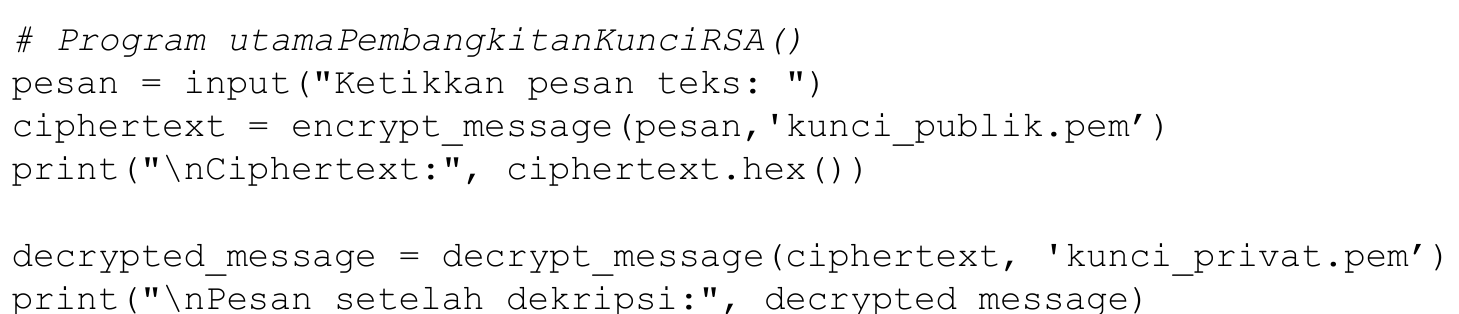
\includegraphics[width=159.60mm,height=86.13mm]{images/llm/page_038_img_01.png}%
\end{textblock*}

\newpage

% --- unit llm 39 ---
% === Halaman 39 (llm) ===

\textcolor{red}{\Huge Hasil run program:}

Modulus (n):

129428027742826116391039211608213298025036352427274045813577140837303610752194709849672822185558359556351
4204395989563858870746123164213866342870439398838950774571122577822276949773353786918775265367114619763
645063071246027546346431374448472349995922796838475581888037922993744861645503849968590135966212361877

Kunci publik (e): 65537

Kunci privat (d):

33941358928395796254375934511848964378367530901779352943890480725544397593144726584488858392350764026826103
37479365593966041395743165198531196384150441009635257822727445975978529317762525357198530942766582886
471193718998414639849017606074426517659013697894729544294792499509155880858497866786513172164421031343

Bilangan prima p:

1110981414053221655196244634106544014062846557320204406867712139854739184120501396765588604932990781446
506648660775077857155929078175380364461896770047307

Bilangan prima q:

1164988235677413917319643018305258352043404070598881349399997701942473577022741271001824330641103524095521868
1220857120428308573505974027168304402825125236984511

Ketikkan pesan teks: Jalan-jalan ke pulau Bunaken di Sulawesi Utara

Ciphertext:

6baef110cc8af3fe69ff7606f66e5a2744617b57bca2064da729971266c159877a93a8d3b7ac14afd2fda9920da55acb28684687db0e5
ae45fe7de96ab696784631ed5cc8ca93039a947c87a37e4af6b7a9479ce9ff13ea0b5f1190a666cad77677a4752bc1100362d10b3c
9b8c704b0bf95c431b23decee585da5d0aff72d001

Pesan setelah dekripsi: b'Jalan-jalan ke pulau Bunaken di Sulawesi Utara'

\newpage

% --- unit llm 40 ---
% === Halaman 40 (llm) ===

\textbf{Catatan:}

\vspace{92.07mm}

\begin{enumerate}
  \item Di dalam pustaka \texttt{Crypto.PublicKey.RSA} dari \texttt{PyCryptodome}, fungsi \texttt{RSA.generate()} secara default menggunakan kunci publik $e = 0x10001$ (atau 65537 dalam desimal), karena nilai ini dianggap aman dan efisien.
  \item Namun, jika Anda ingin menspesifikasikan nilai $e$ lain (misalnya 97 atau nilai lainnya), Anda bisa menentukan nilai $e$ saat memanggil \texttt{RSA.generate()}, seperti berikut:
  
  \vspace{10mm}
  
  \item Pastikan nilai $e$ yang dipilih adalah \textbf{bilangan ganjil}, serta tidak terlalu kecil untuk menghindari potensi kelemahan RSA.
\end{enumerate}

% deskripsi: Potongan kode Python yang menunjukkan cara menggunakan PyCryptodome untuk menghasilkan kunci RSA dengan nilai e kustom.
% bbox normalisasi: [0.1900, 0.4800, 0.5600, 0.7900]
\begin{textblock*}{77.70mm}(39.90mm,142.56mm)
\noindent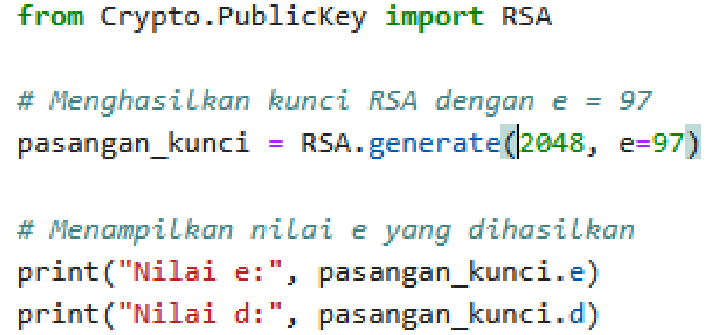
\includegraphics[width=77.70mm,height=92.07mm]{images/llm/page_040_img_01.png}%
\end{textblock*}

\newpage

% --- unit llm 41 ---
% === Halaman 41 (llm) ===

% (tidak ada teks dari model)

% deskripsi: Screenshot kode program Python untuk menghasilkan kunci RSA menggunakan library Crypto.PublicKey dengan parameter e = 97 dan panjang kunci 2048 bit, serta menampilkan hasil nilai e dan d.
% bbox normalisasi: [0.0000, 0.1700, 1.0000, 0.7200]
\begin{textblock*}{210.00mm}(0.00mm,50.49mm)
\noindent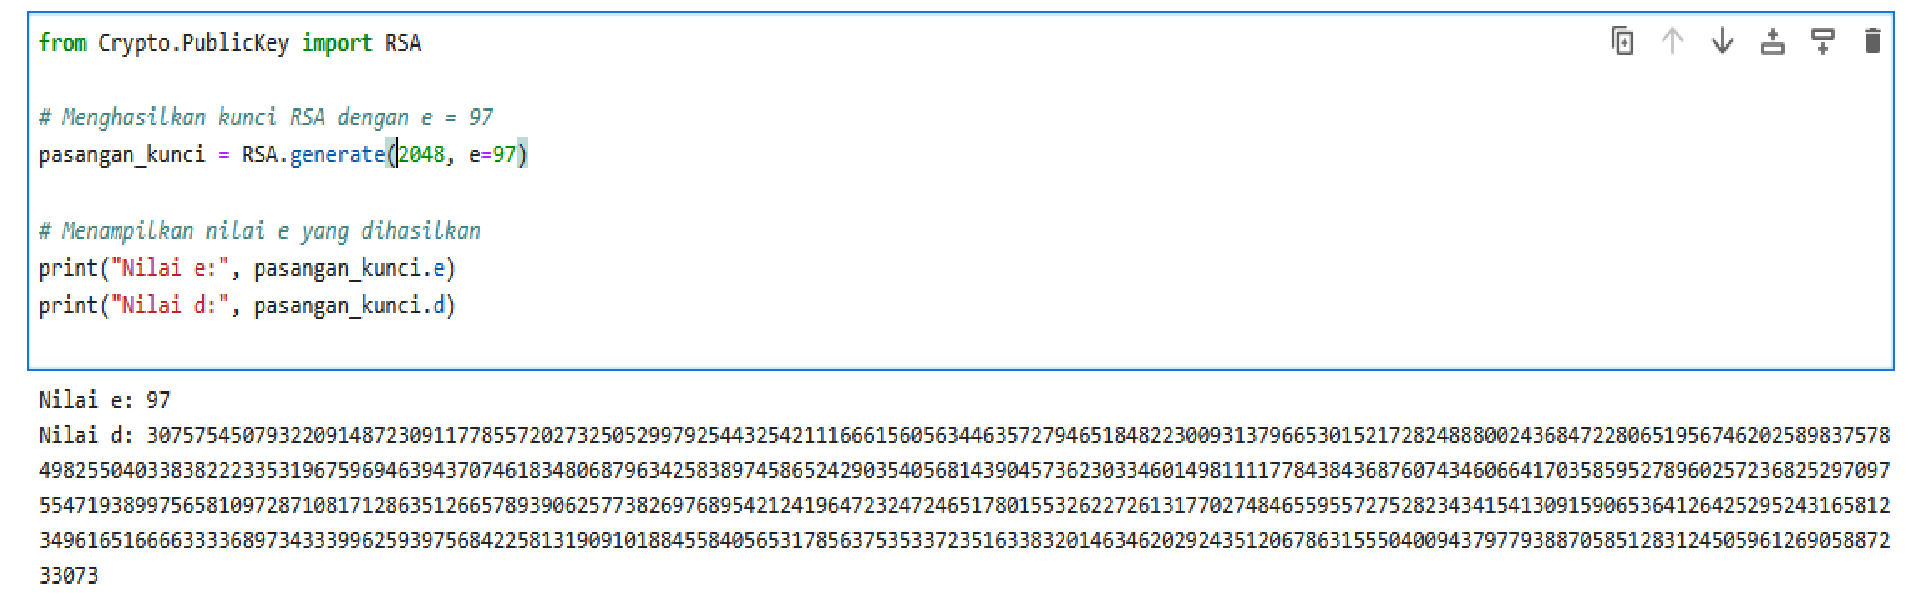
\includegraphics[width=210.00mm,height=163.35mm]{images/llm/page_041_img_01.png}%
\end{textblock*}

\newpage

% --- unit llm 42 ---
% === Halaman 42 (llm) ===

3. Kode Program RSA Python (3)

\vspace{240.57mm}

\begin{verbatim}
from Crypto.PublicKey import RSA
from Crypto.Cipher import PKCS1_OAEP

def PembangkitanKunciRSA(filekuncipublik, filekunciprivat):
    # Buat kunci RSA
    key = RSA.generate(1024)
    kunci_publik = key.publickey()

    # Tampilkan informasi kunci
    print("Modulus (n):", key.n)
    print("Kunci publik (e):", key.e)
    print("Kunci privat (d):", key.d)
    print("Bilangan prima p:", key.p)
    print("Bilangan prima q:", key.q)

    #Simpan kunci publik dan kunci privat ke dalam dua file kunci berbeda, format PEM
    with open(filekuncipublik, "wb") as file:
        file.write(kunci_publik.exportKey('PEM'))
        file.close()

    with open(filekunciprivat, "wb") as file:
        file.write(key.exportKey('PEM','passwordku'))  # Password bisa diubah
        file.close()
\end{verbatim}

% deskripsi: Screenshot potongan kode program Python untuk pembangkitan kunci RSA menggunakan library Crypto.
% bbox normalisasi: [0.0700, 0.1200, 0.9300, 0.9300]
\begin{textblock*}{180.60mm}(14.70mm,35.64mm)
\noindent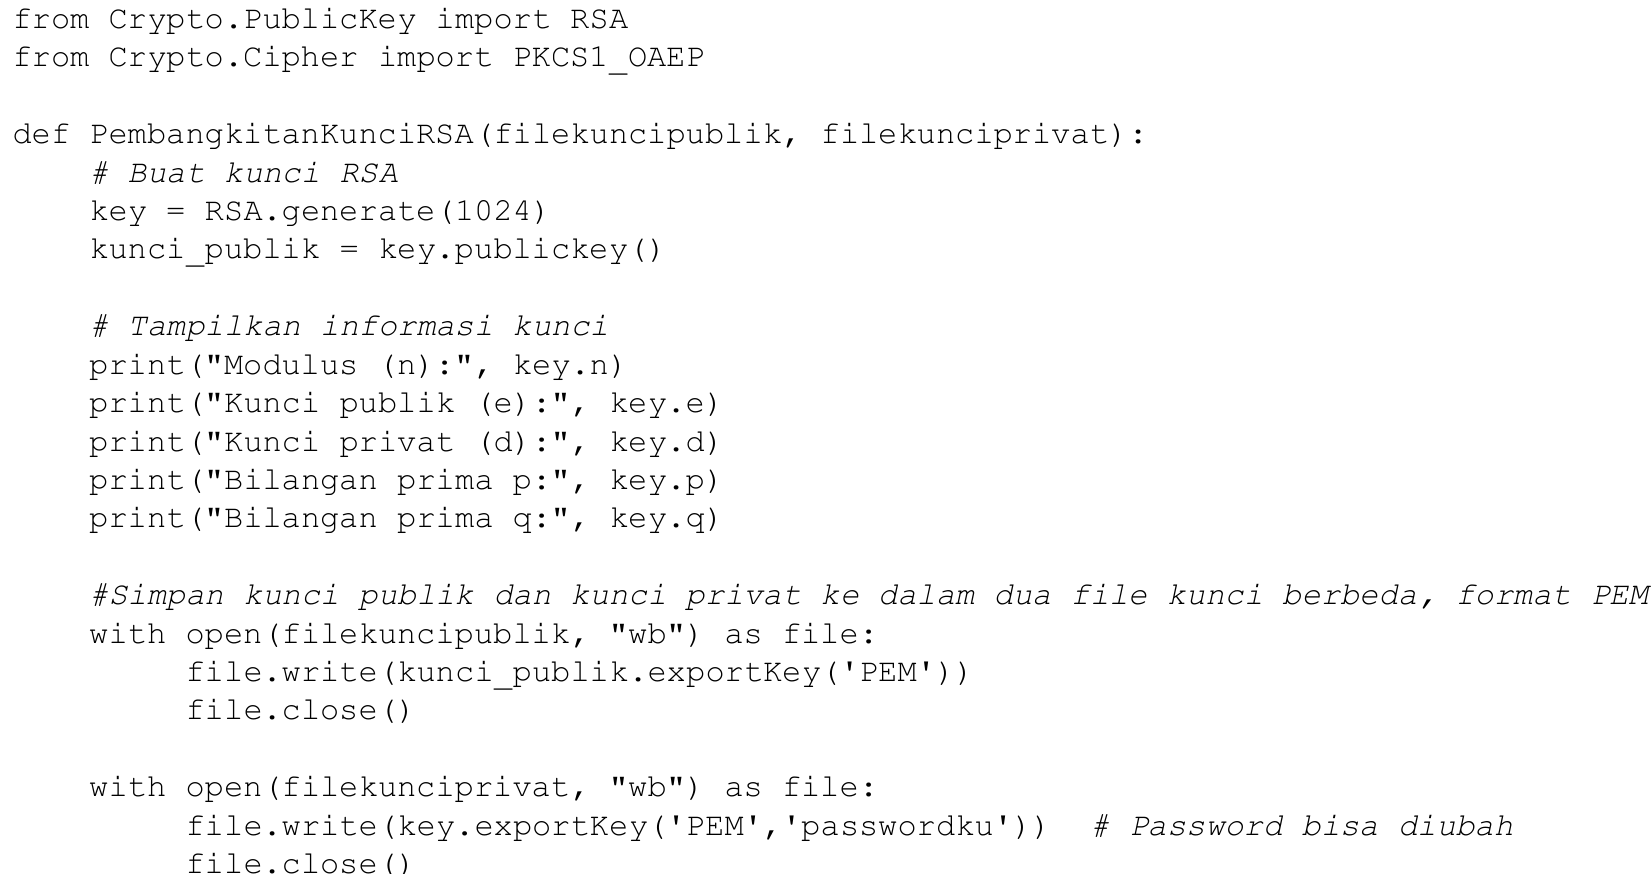
\includegraphics[width=180.60mm,height=240.57mm]{images/llm/page_042_img_01.png}%
\end{textblock*}

\newpage

% --- unit llm 43 ---
% === Halaman 43 (llm) ===

\begin{verbatim}
def encrypt_message(message, file_kunci):
    #Enkripsi pesan
    with open(file_kunci, "rb") as file:
        kunci_publik = RSA.importKey(file.read())

\vspace{193.05mm}

    RSA_cipher = PKCS1_OAEP.new(kunci_publik)
    ciphertext = RSA_cipher.encrypt(message.encode())
    return ciphertext

def decrypt_message(ciphertext, file_kunci):
    #Dekripsi pesan
    with open(file_kunci, "rb") as file:
        kunci_privat = RSA.importKey(file.read(), 'passwordku')

    RSA_cipher = PKCS1_OAEP.new(kunci_privat)
    plaintext = RSA_cipher.decrypt(ciphertext)
    return plaintext
\end{verbatim}

% deskripsi: Screenshot potongan kode Python untuk enkripsi dan dekripsi pesan menggunakan algoritma RSA dengan padding PKCS1_OAEP.
% bbox normalisasi: [0.1100, 0.1500, 0.8300, 0.8000]
\begin{textblock*}{151.20mm}(23.10mm,44.55mm)
\noindent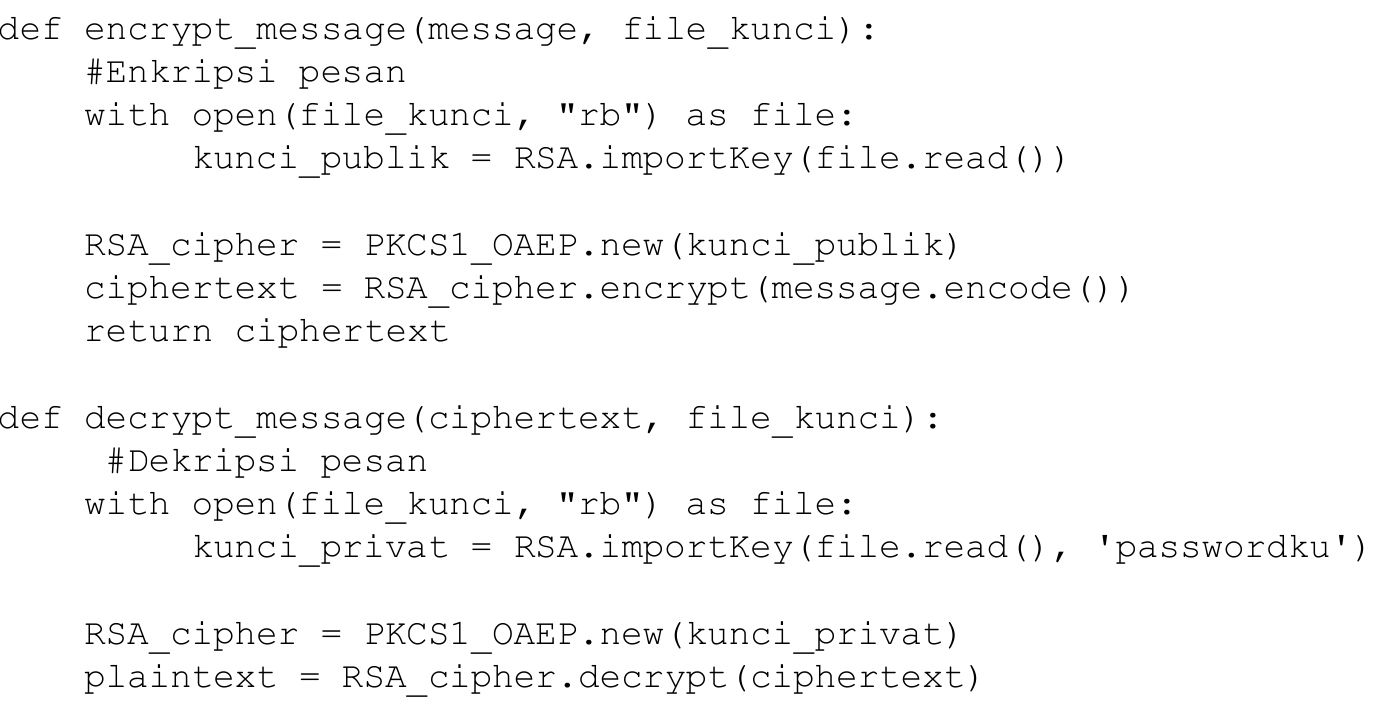
\includegraphics[width=151.20mm,height=193.05mm]{images/llm/page_043_img_01.png}%
\end{textblock*}

\newpage

% --- unit llm 44 ---
% === Halaman 44 (llm) ===

# Program utama

#Alice membangkitkan kunci publik dan kunci privatnya\nprint("\nKUNCI PUBLIK DAN KUNCI PRIVAT ALICE:")\nPembangkitanKunciRSA('kunci\_publik\_Alice.pem', 'kunci\_privat\_Alice.pem')

\vspace{169.29mm}

#Bob membangkitkan kunci publik dan kunci privatnya\nprint("\nKUNCI PUBLIK DAN KUNCI PRIVAT BOB:")\nPembangkitanKunciRSA("kunci\_publik\_Bob.pem", "kunci\_privat\_Bob.pem")

#Bob mengirim pesan kepada Alice\npesan = input("\nBob, ketikkan pesan teks buat Alice: ")

#Bob mengenkripsi pesan dengan menggunakan kunci publik Alice\nciphertext = encrypt\_message(pesan, 'kunci\_publik\_Alice.pem')\nprint("\nCiphertext (dari Bob):", ciphertext.hex())

#Alice mendekripsi ciphertext dari Bob menggunakab kunci privatnya sendiri\n(kunci privat Alice)\ndecrypted\_message = decrypt\_message(ciphertext, 'kunci\_privat\_Alice.pem')\nprint("\nPesan setelah dekripsi oleh Alice:", decrypted\_message)

% deskripsi: Screenshot potongan kode program Python yang mengilustrasikan proses enkripsi dan dekripsi menggunakan algoritma RSA antara dua pengguna, Alice dan Bob.
% bbox normalisasi: [0.0900, 0.3000, 0.9300, 0.8700]
\begin{textblock*}{176.40mm}(18.90mm,89.10mm)
\noindent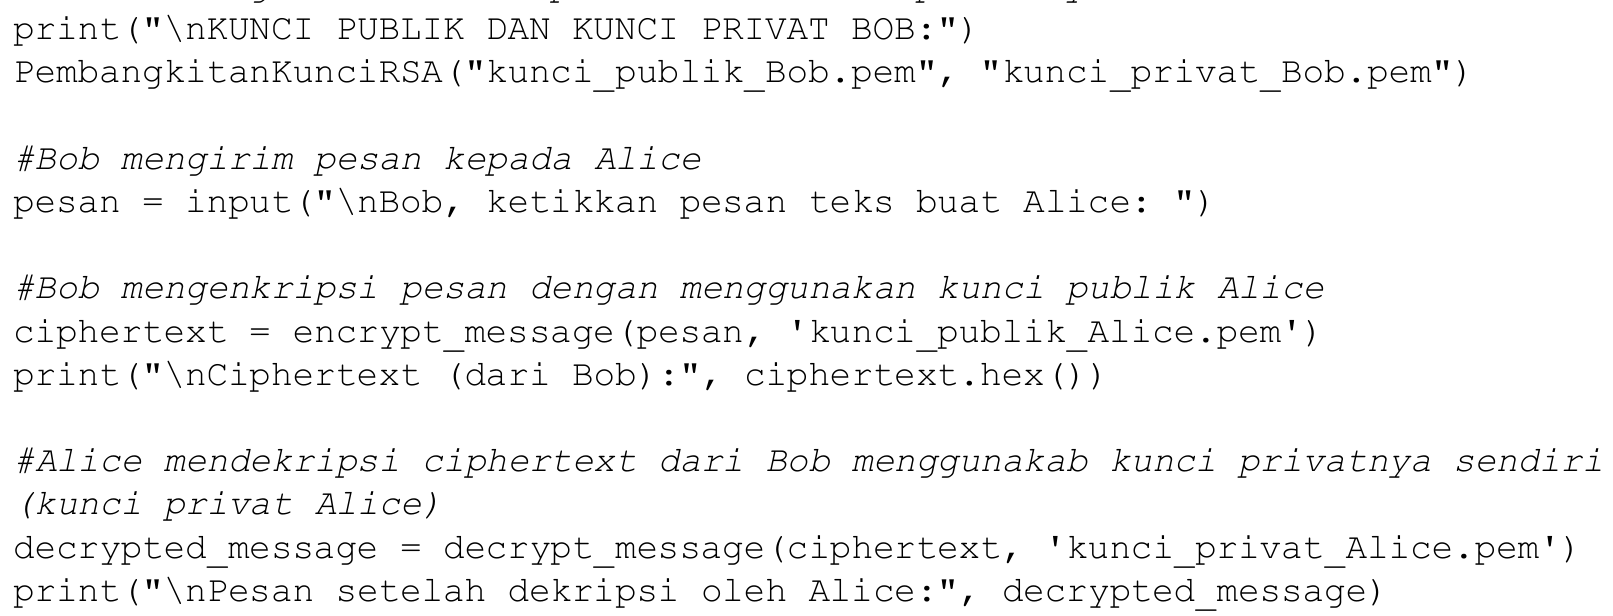
\includegraphics[width=176.40mm,height=169.29mm]{images/llm/page_044_img_01.png}%
\end{textblock*}

\newpage

% --- unit llm 45 ---
% === Halaman 45 (llm) ===

\begin{verbatim}
#Alice membalas pesan dari Bob, dengan mengirimim pesan berikut:
pesan = input("\nAlice, ketikkan pesan teks buat Bob: ")

#Alice mengenkripsi pesan dengan menggunakan kunci publik Bob
ciphertext = encrypt_message(pesan, 'kunci_publik_Bob.pem')
print("\nCiphertext (dari Alice):", ciphertext.hex())

#Bob mendekripsi ciphertext dari Alice menggunakab kunci privatnya
sendiri (kunci privat Bob)
decrypted_message = decrypt_message(ciphertext, 'kunci_privat_Bob.pem')
print("\nPesan setelah dekripsi oleh Bob:", decrypted_message)
\end{verbatim}

\newpage

% --- unit llm 46 ---
% === Halaman 46 (llm) ===

\textcolor{red}{Hasil run program:}

KUNCI PUBLIK DAN KUNCI PRIVAT ALICE:

Modulus (n):
\[
\begin{aligned}
&12132448764569524967124728413902431780482235091094867693654938954713626107169684397247814 \\
&12474343076775995103804018887666258583541197752662283643205966312416809471671556500234930 \\
&957303088959837811895781631530720919977085954392832689243057969416275830939335223499796 \\
&217037614957603521783374145640784114434563
\end{aligned}
\]

Kunci publik (e): 65537

Kunci privat (d):
\[
\begin{aligned}
&33939336153690478823253025658006609392481749750025060813027838854858041304623476908648538 \\
&3246908970119455712059525856724406167242213121159324777165476355380842538062809524569904 \\
&72059874731060015045340299556018306078460861526542442894603564004740903003998810068546432 \\
&010940711141178270308307312496291007873
\end{aligned}
\]

Bilangan prima p:
\[
\begin{aligned}
&10266126063909086853415825065972364144507017404008150872006369257162348806926981473326304 \\
&59853도326382555815580890529498086596307687781847774230340012781016929
\end{aligned}
\]

Bilangan prima q:
\[
\begin{aligned}
&11817942512143464363674809387674657751200321120697482150084327982300021312243111046301987 \\
&4793519954251825050851664698261250524580829201805990724029021874147
\end{aligned}
\]

\newpage

% --- unit llm 47 ---
% === Halaman 47 (llm) ===

KUNCI PUBLIK DAN KUNCI PRIVAT BOB:\\
Modulus (n):\\
16684994592485789138232294581326251341129318223836974845260523372874568341196667883164\n769671350993682836723086797587170075503900188700167822316544899938712936536455510465493\n707365982892129712589859541722763559046642574039480605479421279179816357971677653115772\n159590836882786763184690297360998353712774925663

Kunci publik (e): 65537

Kunci privat (d):\\
496652079400310172041539222529641654510086018571282131510649295811226800006113279073619\n2268106131169819764093503704954684198686251259771254997596954072967012215308767218906732\n622103339294066623572886670148185902779533190873629122112316955478376017380077949395915\n652549207566114236209976478028439266112657746093953

Bilangan prima p:\\
127568999117375604154435685620126106245530350635499363428145130663430764832634501183152\n49363209417884220088720467829317972477109073296012607939188116565711\\
Bilangan prima q:\\
1307919215850929276296196781541821885348837776304964807967608240600324455832787407102228\n490890295595849634046551071349701708960132858083226877641768264965233

\newpage

% --- unit llm 48 ---
% === Halaman 48 (llm) ===

Bob, ketikkan pesan teks buat Alice: Alice, apa kabar, sayang? Sudah lama kita tidak bertemu. Bagaimana kabarmu?
Sehat?

Ciphertext (dari Bob):

33142cf0694daef5cc6d72dcdacafbec647e1cf55889b9a9125c7b09d0168da7bc2b27651d113754907776f818d054e925
bfa0e4b6968f9586bd553bb9db901aea32e71dd8328a9250fbd171ec485b45e70041515b12fe82742958d0601e274dca
7f8f404a7a7d6d3209cae1b0d401d28c9aeba0b9f128d2ea10ab257582e7ff

Pesan setelah dekripsi oleh Alice: b'Alice, apa kabar, sayang? Sudah lama kita tidak bertemu. Bagaimana kabarmu?
Sehat?'

Alice, ketikkan pesan teks buat Bob: Alhamdulillah, sehat Bob. Kamu sekarang di mana? Masih bertugas di
Balikpapan?

Ciphertext (dari Alice):

bd820c7dd21d06f284da43725f3319af6fa058146c2eaf7b95a72cdb4f7123581a9d7e2145a446286f4c211082f6a33f671
db427e843b550c925e3cc22812cc50c79056be69dda98452cc64fd4a3b187ea884feee8a4810eca66f149fd700efa14b0
8f4ce8d9a64749e63cfe2a7cedddf4a21435b83b0d62baedc282902856f

Pesan setelah dekripsi oleh Bob: b'Alhamdulillah, sehat Bob. Kamu sekarang di mana? Masih bertugas di Balikpapan?'

\newpage

% --- unit llm 49 ---
% === Halaman 49 (llm) ===

\begin{center}
\huge Lampiran Bilangan Prima
\end{center}

\newpage

% --- unit llm 50 ---
% === Halaman 50 (llm) ===

\vspace{204.93mm}

Di bawah ini daftar 10.000 bilangan prima pertama (Sumber: http://primes.utm.edu):

\vspace{5mm}

% deskripsi: Daftar angka-angka bilangan prima yang disusun dalam format kolom
% bbox normalisasi: [0.0800, 0.1900, 0.8200, 0.8800]
\begin{textblock*}{155.40mm}(16.80mm,56.43mm)
\noindent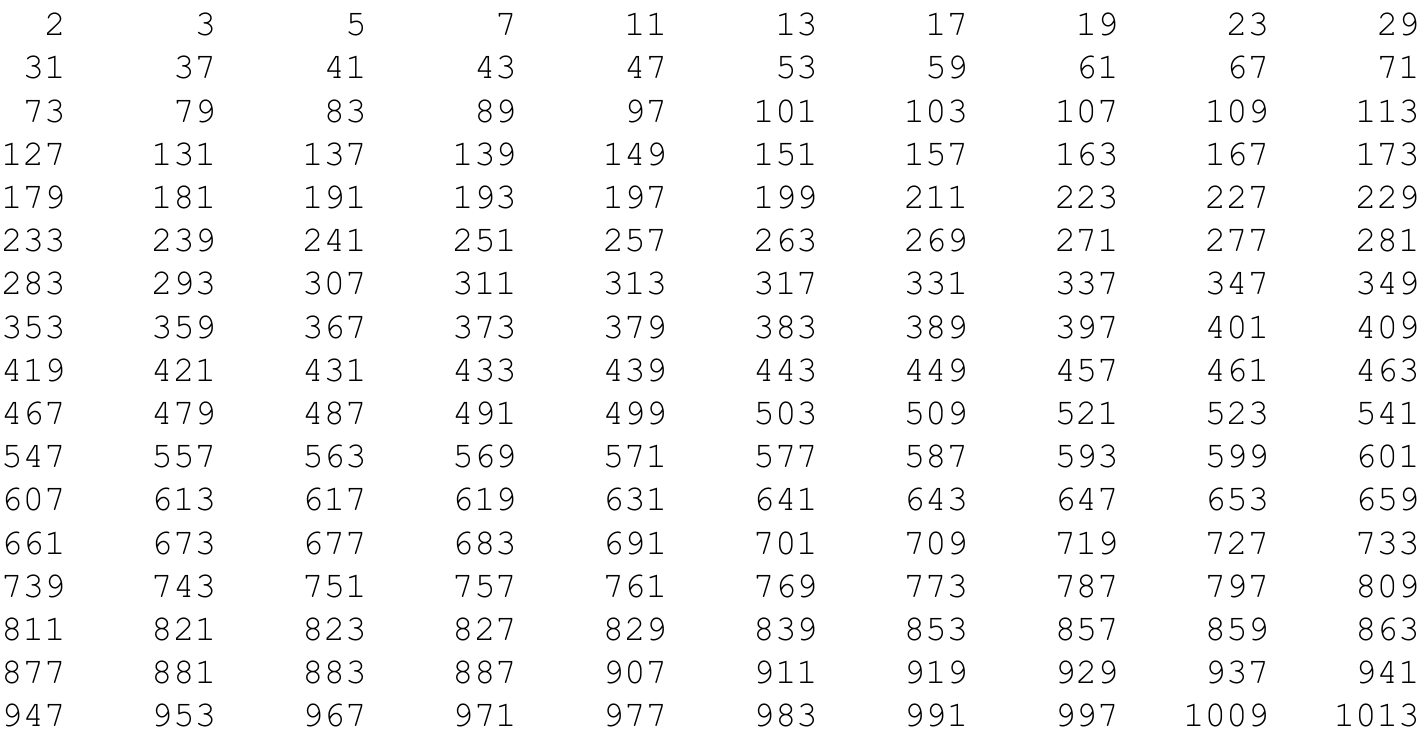
\includegraphics[width=155.40mm,height=204.93mm]{images/llm/page_050_img_01.png}%
\end{textblock*}

\newpage

% --- unit llm 51 ---
% === Halaman 51 (llm) ===

\begin{tabular}{rrrrrrrrrr}
1019 & 1021 & 1031 & 1033 & 1039 & 1049 & 1051 & 1061 & 1063 & 1069 \\
1087 & 1091 & 1093 & 1097 & 1103 & 1109 & 1117 & 1123 & 1129 & 1151 \\
1153 & 1163 & 1171 & 1181 & 1187 & 1193 & 1201 & 1213 & 1217 & 1223 \\
1229 & 1231 & 1237 & 1249 & 1259 & 1277 & 1279 & 1283 & 1289 & 1291 \\
1297 & 1301 & 1303 & 1307 & 1319 & 1321 & 1327 & 1361 & 1367 & 1373 \\
1381 & 1399 & 1409 & 1423 & 1427 & 1429 & 1433 & 1439 & 1447 & 1451 \\
1453 & 1459 & 1471 & 1481 & 1483 & 1487 & 1489 & 1493 & 1499 & 1511 \\
1523 & 1531 & 1543 & 1549 & 1553 & 1559 & 1567 & 1571 & 1579 & 1583 \\
1597 & 1601 & 1607 & 1609 & 1613 & 1619 & 1621 & 1627 & 1637 & 1657 \\
1663 & 1667 & 1669 & 1693 & 1697 & 1699 & 1709 & 1721 & 1723 & 1733 \\
1741 & 1747 & 1753 & 1759 & 1777 & 1783 & 1787 & 1789 & 1801 & 1811 \\
1823 & 1831 & 1847 & 1861 & 1867 & 1871 & 1873 & 1877 & 1879 & 1889 \\
1901 & 1907 & 1913 & 1931 & 1933 & 1949 & 1951 & 1973 & 1979 & 1987 \\
1993 & 1997 & 1999 & 2003 & 2011 & 2017 & 2027 & 2029 & 2039 & 2053 \\
2063 & 2069 & 2081 & 2083 & 2087 & 2089 & 2099 & 2111 & 2113 & 2129 \\
2131 & 2137 & 2141 & 2143 & 2153 & 2161 & 2179 & 2203 & 2207 & 2213 \\
2221 & 2237 & 2239 & 2243 & 2251 & 2267 & 2269 & 2273 & 2281 & 2287 \\
2293 & 2297 & 2309 & 2311 & 2333 & 2339 & 2341 & 2347 & 2351 & 2357
\end{tabular}

\newpage

% --- unit llm 52 ---
% === Halaman 52 (llm) ===

\begin{tabular}{ccccccccc}
2371 & 2377 & 2381 & 2383 & 2389 & 2393 & 2399 & 2411 & 2417 & 2423 \\
2437 & 2441 & 2447 & 2459 & 2467 & 2473 & 2477 & 2503 & 2521 & 2531 \\
2539 & 2543 & 2549 & 2551 & 2557 & 2579 & 2591 & 2593 & 2609 & 2617 \\
2621 & 2633 & 2647 & 2657 & 2659 & 2663 & 2671 & 2677 & 2683 & 2687 \\
2689 & 2693 & 2699 & 2707 & 2711 & 2713 & 2719 & 2729 & 2731 & 2741 \\
2749 & 2753 & 2767 & 2777 & 2789 & 2791 & 2797 & 2801 & 2803 & 2819 \\
2833 & 2837 & 2843 & 2851 & 2857 & 2861 & 2879 & 2887 & 2897 & 2903 \\
2909 & 2917 & 2927 & 2939 & 2953 & 2957 & 2963 & 2969 & 2971 & 2999 \\
3001 & 3011 & 3019 & 3023 & 3037 & 3041 & 3049 & 3061 & 3067 & 3079 \\
3083 & 3089 & 3109 & 3119 & 3121 & 3137 & 3163 & 3167 & 3169 & 3181 \\
3187 & 3191 & 3203 & 3209 & 3217 & 3221 & 3229 & 3251 & 3253 & 3257 \\
3259 & 3271 & 3299 & 3301 & 3307 & 3313 & 3319 & 3323 & 3329 & 3331 \\
3343 & 3347 & 3359 & 3361 & 3371 & 3373 & 3389 & 3391 & 3407 & 3413 \\
3433 & 3449 & 3457 & 3461 & 3463 & 3467 & 3469 & 3491 & 3499 & 3511 \\
3517 & 3527 & 3529 & 3533 & 3539 & 3541 & 3547 & 3557 & 3559 & 3571 \\
3581 & 3583 & 3593 & 3607 & 3613 & 3617 & 3623 & 3631 & 3637 & 3643 \\
3659 & 3671 & 3673 & 3677 & 3691 & 3697 & 3701 & 3709 & 3719 & 3727 \\
3733 & 3739 & 3761 & 3767 & 3769 & 3779 & 3793 & 3797 & 3803 & 3821 \\
3823 & 3833 & 3847 & 3851 & 3853 & 3863 & 3877 & 3881 & 3889 & 3907 \\
3911 & 3917 & 3919 & 3923 & 3929 & 3931 & 3943 & 3947 & 3967 & 3989
\end{tabular}

\newpage

% --- unit llm 53 ---
% === Halaman 53 (llm) ===

\begin{tabular}{rrrrrrrrrr}
4001 & 4003 & 4007 & 4013 & 4019 & 4021 & 4027 & 4049 & 4051 & 4057 \\
4073 & 4079 & 4091 & 4093 & 4099 & 4111 & 4127 & 4129 & 4133 & 4139 \\
4153 & 4157 & 4159 & 4177 & 4201 & 4211 & 4217 & 4219 & 4229 & 4231 \\
4241 & 4243 & 4253 & 4259 & 4261 & 4271 & 4273 & 4283 & 4289 & 4297 \\
4327 & 4337 & 4339 & 4349 & 4357 & 4363 & 4373 & 4391 & 4397 & 4409 \\
4421 & 4423 & 4441 & 4447 & 4451 & 4457 & 4463 & 4481 & 4483 & 4493 \\
4507 & 4513 & 4517 & 4519 & 4523 & 4547 & 4549 & 4561 & 4567 & 4583 \\
4591 & 4597 & 4603 & 4621 & 4637 & 4639 & 4643 & 4649 & 4651 & 4657 \\
4663 & 4673 & 4679 & 4691 & 4703 & 4721 & 4723 & 4729 & 4733 & 4751 \\
4759 & 4783 & 4787 & 4789 & 4793 & 4799 & 4801 & 4813 & 4817 & 4831 \\
4861 & 4871 & 4877 & 4889 & 4903 & 4909 & 4919 & 4931 & 4933 & 4937 \\
4943 & 4951 & 4957 & 4967 & 4969 & 4973 & 4987 & 4993 & 4999 & 5003 \\
5009 & 5011 & 5021 & 5023 & 5039 & 5051 & 5059 & 5077 & 5081 & 5087 \\
5099 & 5101 & 5107 & 5113 & 5119 & 5147 & 5153 & 5167 & 5171 & 5179 \\
5189 & 5197 & 5209 & 5227 & 5231 & 5233 & 5237 & 5261 & 5273 & 5279 \\
5281 & 5297 & 5303 & 5309 & 5323 & 5333 & 5347 & 5351 & 5381 & 5387 \\
5393 & 5399 & 5407 & 5413 & 5417 & 5419 & 5431 & 5437 & 5441 & 5443 \\
5449 & 5471 & 5477 & 5479 & 5483 & 5501 & 5503 & 5507 & 5519 & 5521 \\
5527 & 5531 & 5557 & 5563 & 5569 & 5573 & 5581 & 5591 & 5623 & 5639 \\
5641 & 5647 & 5651 & 5653 & 5657 & 5659 & 5669 & 5683 & 5689 & 5693 \\
5701 & 5711 & 5717 & 5737 & 5741 & 5743 & 5749 & 5779 & 5783 & 5791 \\
5801 & 5807 & 5813 & 5821 & 5827 & 5839 & 5843 & 5849 & 5851 & 5857 \\
\end{tabular}

\newpage

% --- unit llm 54 ---
% === Halaman 54 (llm) ===

\begin{tabular}{llllllllll}
5861 & 5867 & 5869 & 5879 & 5881 & 5897 & 5903 & 5923 & 5927 & 5939 \\
5953 & 5981 & 5987 & 6007 & 6011 & 6029 & 6037 & 6043 & 6047 & 6053 \\
6067 & 6073 & 6079 & 6089 & 6091 & 6101 & 6113 & 6121 & 6131 & 6133 \\
6143 & 6151 & 6163 & 6173 & 6197 & 6199 & 6203 & 6211 & 6217 & 6221 \\
6229 & 6247 & 6257 & 6263 & 6269 & 6271 & 6277 & 6287 & 6299 & 6301 \\
6311 & 6317 & 6323 & 6329 & 6337 & 6343 & 6353 & 6359 & 6361 & 6367 \\
6373 & 6379 & 6389 & 6397 & 6421 & 6427 & 6449 & 6451 & 6469 & 6473 \\
6481 & 6491 & 6521 & 6529 & 6547 & 6551 & 6553 & 6563 & 6569 & 6571 \\
6577 & 6581 & 6599 & 6607 & 6619 & 6637 & 6653 & 6659 & 6661 & 6673 \\
6679 & 6689 & 6691 & 6701 & 6703 & 6709 & 6719 & 6733 & 6737 & 6761 \\
6763 & 6779 & 6781 & 6791 & 6793 & 6803 & 6823 & 6827 & 6829 & 6833 \\
6841 & 6857 & 6863 & 6869 & 6871 & 6883 & 6899 & 6907 & 6911 & 6917 \\
6947 & 6949 & 6959 & 6961 & 6967 & 6971 & 6977 & 6983 & 6991 & 6997 \\
7001 & 7013 & 7019 & 7027 & 7039 & 7043 & 7057 & 7069 & 7079 & 7103 \\
7109 & 7121 & 7127 & 7129 & 7151 & 7159 & 7177 & 7187 & 7193 & 7207 \\
7211 & 7213 & 7219 & 7229 & 7237 & 7243 & 7247 & 7253 & 7283 & 7297 \\
7307 & 7309 & 7321 & 7331 & 7333 & 7349 & 7351 & 7369 & 7393 & 7411 \\
7417 & 7433 & 7451 & 7457 & 7459 & 7477 & 7481 & 7487 & 7489 & 7499 \\
7507 & 7517 & 7523 & 7529 & 7537 & 7541 & 7547 & 7549 & 7559 & 7561 \\
7573 & 7577 & 7583 & 7589 & 7591 & 7603 & 7607 & 7621 & 7639 & 7643 \\
7649 & 7669 & 7673 & 7681 & 7687 & 7691 & 7699 & 7703 & 7717 & 7723 \\
7727 & 7741 & 7753 & 7757 & 7759 & 7789 & 7793 & 7817 & 7823 & 7829 \\
7841 & 7853 & 7867 & 7873 & 7877 & 7879 & 7883 & 7901 & 7907 & 7919
\end{tabular}

\end{document}
